\documentclass[9pt,twocolumn,twoside,lineno]{pnas-new}
% Use the lineno option to display guide line numbers if required.

\templatetype{pnasresearcharticle} % Choose template 
% {pnasresearcharticle} = Template for a two-column research article
% {pnasmathematics} %= Template for a one-column mathematics article
% {pnasinvited} %= Template for a PNAS invited submission

\title{Does reducing Malaria's burden cause economic growth, or does growth reduce Malaria?}

% Use letters for affiliations, numbers to show equal authorship (if applicable) and to indicate the corresponding author
\author[a,b,1]{Joe Brew}

\affil[a]{Barcelona Institute for Global Health: c/ Rosselló, 132, 5è 2a. 08036, Barcelona, Catalonia}
\affil[b]{VU University Amsterdam: De Boelelaan 1105, 1081 HV Amsterdam, Netherlands}

% Please give the surname of the lead author for the running footer
\leadauthor{Brew} 

% Please add here a significance statement to explain the relevance of your work
\significancestatement{Malaria is a "disease of poverty" but the extent to which Malaria is the cause or effect of poverty is not fully understood. Identifying the direction of the causal relationship between health and wealth is vital to knowing whether development interventions in poor, Malaria-endemic societies should target the disease or the poverty. We analyzed the relationship between GDP and the prevalence of Plasmodium falciparum among children in 27 Malaria-endemic African countries, and identified health to wealth as the primary causal pathway. Our findings suggest that in countries with a high burden of Malaria, targeting the disease directly through public health interventions may lead to economic growth.}

% Please include corresponding author, author contribution and author declaration information
\authorcontributions{Author contributions: J.B. and E.S. designed research; J.B. gathered and processed data; J.B. and E.S. analyzed
data; J.B. and E.S. wrote the paper}
\authordeclaration{The authors declare no conflicts of interest}
\correspondingauthor{\textsuperscript{1}E-mail: joebrew@gmail.com}

% Keywords are not mandatory, but authors are strongly encouraged to provide them. If provided, please include two to five keywords, separated by the pipe symbol, e.g:
\keywords{Malaria $|$ Economics $|$ Development $|$ Growth $|$ Causality} 

\begin{abstract}
The correlation between poverty and Malaria endemicity has been well established, but causal directionality has not. Understanding the extent to which Malaria causes economic stagnation, and vice-versa, is important for an efficient allotment of development resources. Using 15 years of panel data from 27 Malaria-endemic Sub-Saharan African countries, we employ an instrumented two-step procedure to estimate the response of GDP growth to reductions in Malaria, and vice-versa. Having identified a temporally coherent health-to-wealth pathway, and check for robustness using several methods. Our results are coherent and consistent across methods, suggesting that development-oriented aid and investment in Malaria-endemic countries should prioritize those interventions which reduce Malaria directly.
\end{abstract}

\dates{This manuscript was compiled on \today}
\doi{\url{www.pnas.org/cgi/doi/10.1073/pnas.XXXXXXXXXX}}

\begin{document}

\maketitle
\thispagestyle{firststyle}
\ifthenelse{\boolean{shortarticle}}{\ifthenelse{\boolean{singlecolumn}}{\abscontentformatted}{\abscontent}}{}


\dropcap{M}alaria causes more than a half million deaths worldwide every year \cite{White}. In addition to its devastating health effects, Malaria has a large economic impact.  By reducing one’s ability to work efficiently \cite{Nonvignon2016-vt}, if at all, Malaria imposes a large financial cost on the infected \cite{Asenso-Okyere1997-wj} \cite{Ajani2010-dd}, and the toll trickles upwards to society at large \cite{Sachs2002-ig}. Not only does Malaria likely has a negative effect on GDP and growth \cite{McCarthy2000-wl, Orem2012-kr, Hong2011-sa, Sachs2002-ig}, in a classic feedback loop, low growth can keep societies in a resource-scarce state making interventions which target the control or elimination of Malaria difficult \cite{White, Purdy2013-rt, Howard2017-pk, Phillips1998-ky}. 

The correlation between poverty and Malaria endemicity has been well established, but causal directionality has not. This lack of clarity may partially explain why there are two schools of thought in development circles regarding where resources should be directed. One school argues that a society must be brought out of poverty, after which gains in health are almost inevitable, but prior to which significant health improvements are nearly impossible \cite{Musgrove1996-hm}.  The other argues for a more “holistic” development approach, implicitly calling for resources to be devoted to areas believed to be pre-requiste to wealth acquisition, such as health \cite{Storm2008-dd, Sen_undated-gp}.  Clarke et al. covers this distinction more thoroughly \cite{Clarke_JA2016-ik}.

Though both schools acknowledge that the interaction between health and wealth is bi-directional, understanding the extent to which Malaria’s burden affects the economy, and vice-versa, could shed light on areas where developmentalists should focus in order to break the vicious cycle. Particularly, knowing which kinds of improvements precede the other helps to guide policies which aim to improve well-being in the long-term. Since Malaria’s economic effects are at the macro-scale, a randomized controlled trial to assess the extent to which a controlled shock to the burden of Malaria or the economy is not feasible. Ample experiments and interventions exist at the sub-national level, and occasionally the national level, but these are generally carried out in isolation, lacking the plausible counterfactual with which to compare any observed improvement in Malaria’s burden or economic growth. Additionally, at the sub-national and national levels, the amount of confounding factors (political changes, climate crises, etc.) are too great to isolate causal effects. 

Given the impossibility of parsing these many complex factors at the micro-level, one approach for understanding causal directionality in the Malaria-economy relationship is to focus at the macro-level and on simple temporality (ie, whether changes to the economy tend to preceed changes to Malaria’s burden or vice-versa). By including many countries rather than just one, we cancel out each one’s idiosyncracies, and by carrying out statistical precedence analysis, we can identify a potentially causal trend for further analysis. 

Granger-causation analysis, a form of temporal precedence analysis, is a useful tool for doing this \cite{Granger_undated-wn, Molenaar2018-ss, Koller2016-rv, Granger1896-di, Clarke_JA2016-ik}. In the field of Economics, it is commonly used with panel data to assess the directionality of a bi-directional \cite{Law_2013, Joerding1986, ADALI_2017} or multi-directional \cite{Akbas_2013} relationship. For ths specific link to health and growth, it has been used to examine the causal links between the health status and savings of elderly Europeans \cite{Andreyeva2007-zq}, general health and socieconomic status \cite{Adams2003-wl}, and macro-level development and mortality \cite{Clarke_JA2016-ik}. These studies found causal directionality to be ambiguous. No study, to the authors’ knowledge, has used Granger causality to examine the relationship between Malaria’s burden and GDP. Sachs' seminal study on Malaria's effect on the economy \cite{Sachs2002-ig} focuses largely on societies where elimination of the disease was achieved, and on time-invariant factors such as latitude, distance to coast, colonial history. 

Though Granger's methodology is useful for establishing precedence - a prerequisite of causality - it is not comprehensive enough to provide strong evidence for causality itself. Accordingly, we also employ a two-step instrument variable approach, similar to the one used by Brückner in his study on the relationship between GDP growth and foreign aid, to parse directionality \cite{bruckner2011}. We employ consumer gasoline prices as an instrument for the GDP-to-Malaria causal pathway, and insecticide treated net (ITN) coverage for the opposite. Having estimated the IV models, we then use the residuals from that first step's estimation as an instrument for the second model, in which GDP growth is estimated directly as a function of the prevalence of Malaria, and vice-versa.

Our analysis was carried out on 15 years of data from 27 Malaria-endemic Sub-Saharan African countries. Having identified a temporally coherent health-to-wealth pathway in both the Granger and Brückner approaches, we then carry out two robustness checks. First, we examine a unique health-to-wealth exogenous shock: the introduction of artemisinin-based combination therapy (ACT) and its effect on GDP. Second, we analyze the 2007-8 financial crisis, and its effect on Malaria. 

\section*{Results}

\begin{figure*}%[tbhp] Remove the asterisk to get column width only
\centering
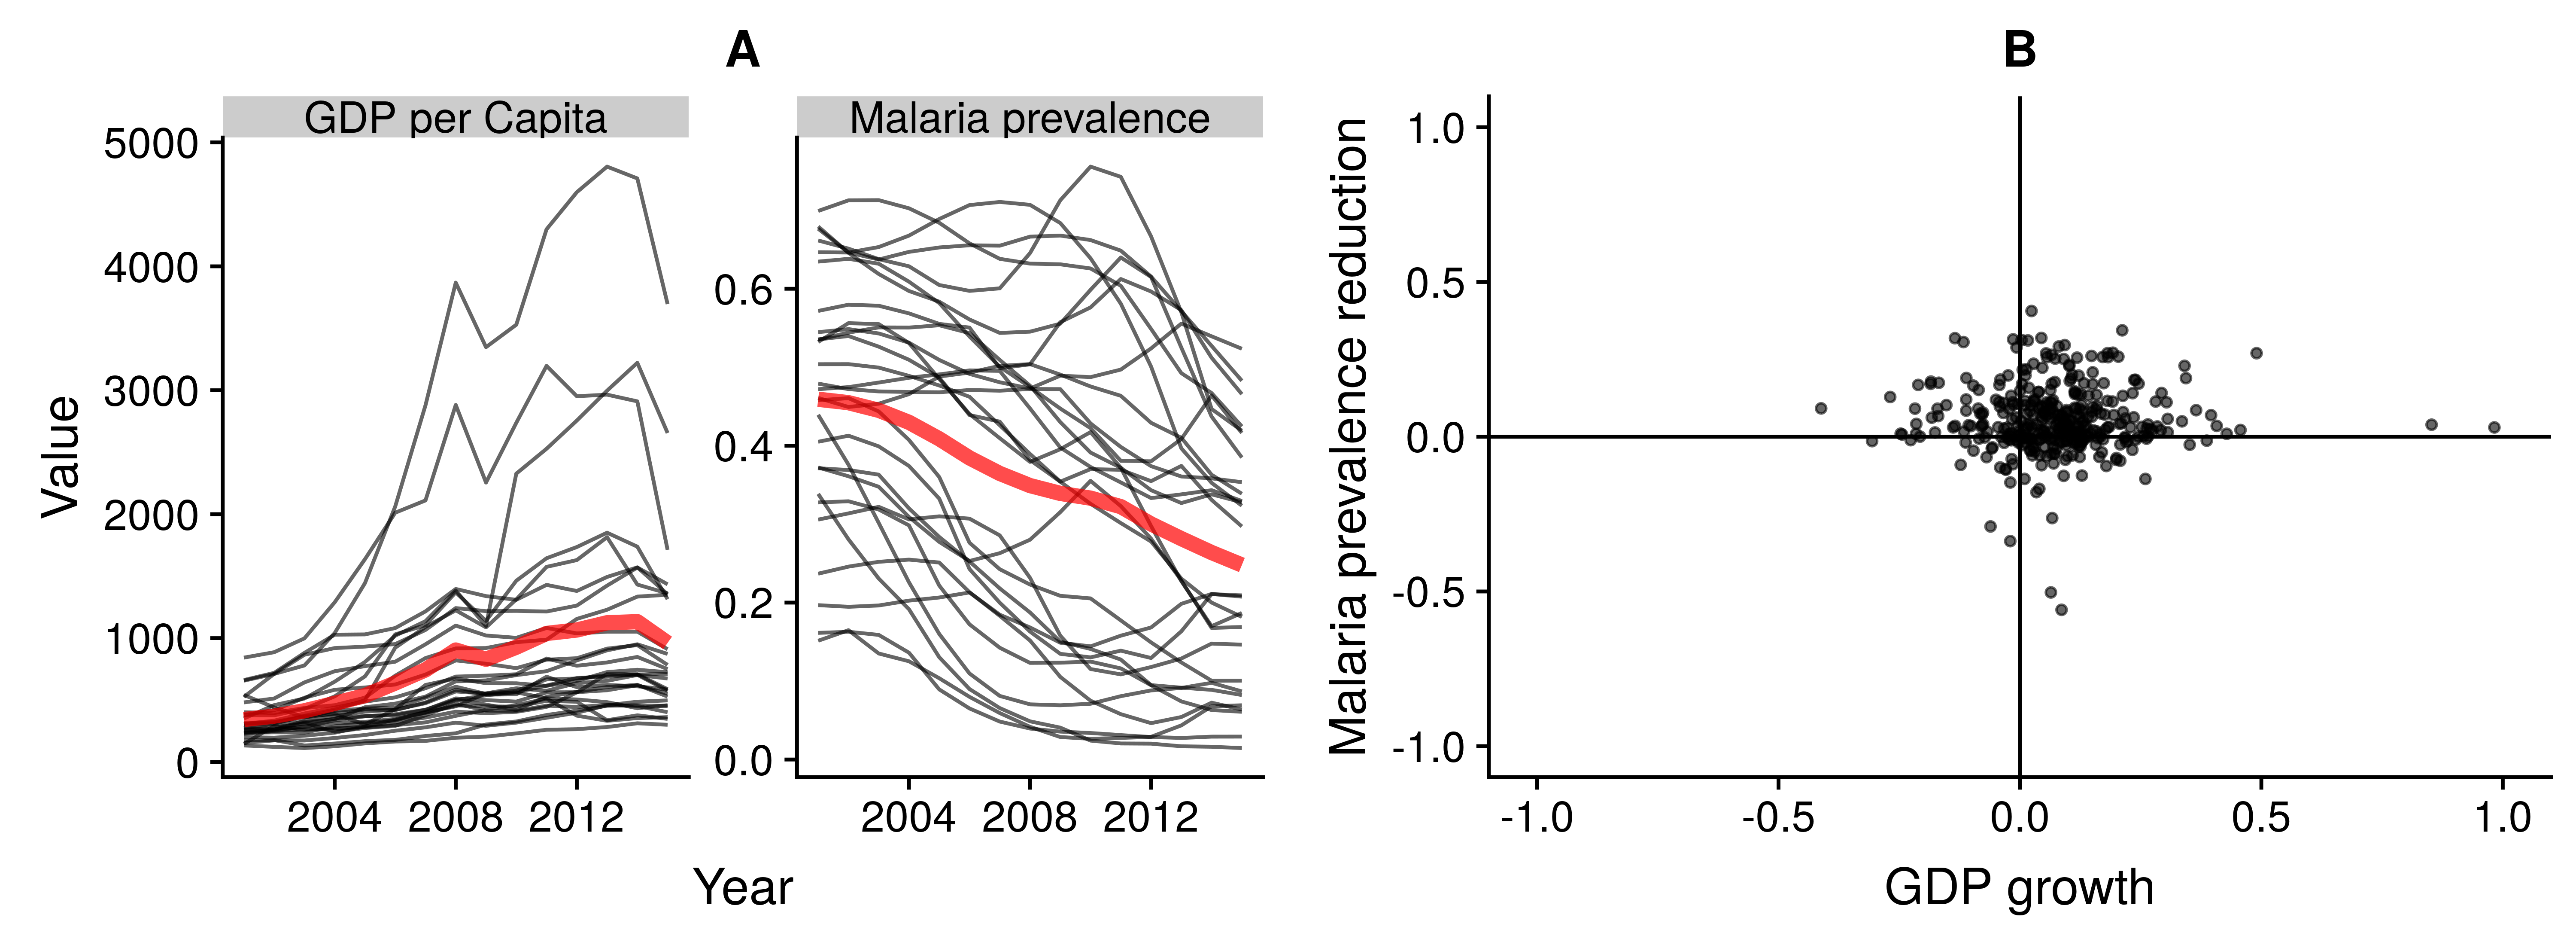
\includegraphics[width=.9\linewidth]{../figures/descriptive}
\caption{A. Country-specific GDP and Malaria prevalence values during observation period (all-country average in black). An overall increasing trend is plainly visible, albeit with a dib in growth following the 2007-8 financial crisis. B. Association of growth (GDP divided by previous year's GDP) and reduction in Malaria prevalence (1 minus prevalence divided by previous year's prevalence). Most observations fall in the upper-right quadrant (ie, increasing GDP and decreasing Malaria prevalence). C. Country-specific GDP-Malaria trajectory, 2000-2015. Each line shows an individual country's 15 year trajectory; the black line is the overall trend. At most times, countries moved rightward (increasing GDP per Capita) and downward (decreasing prevalence of Malaria). D. Countries included in study.}
\label{fig:descriptive}
\end{figure*}


\subsection*{Association of GDP and Malaria prevalence}

We examined the entirety of Sub-Saharan Africa, filtering out countries which had a less than 10\% prevalence of Malaria in 2001 or a GDP per Capita of greater than 10,000 USD at any point in the study period (2001-2015) (Fig. \ref{fig:descriptive}, D). Over the course of the 15 year study period, of the 27 Sub-Saharan African countries which met our inclusion criteria, all but 1 (The Gambia) saw an overall increase in GDP per Capita, and only 1 (Mali) had an overall increase in the prevalence of Malaria. The trajectories of GDP growth and Malaria reduction were hardly uniform, however: of the 405 country-years observed, 104 (26\%) country-years were associated with a reduction in GDP per Capita from the previous year, and 107 (28\%) saw an increase in the prevalence of Malaria relative to the previous year  (Fig. \ref{fig:descriptive}, B). Nonetheless, the overall trend is clear across the continent: over time, as the economy increased, the prevalence of Malaria decreased (Fig. \ref{fig:descriptive}, A and C). For every 1\% decrease in the prevalence of Malaria, GDP per Capita increased on average by 6.2 USD (p<0.01, R-squared=0.03).

However, the association between Malaria prevalence and GDP per Capita appears to be largley mediated by time, and is not evident at any cross-sectional point. We calculated year-specific Pearson's product moment correlation coefficients for the association between GDP per Capita and Malaria prevalence for the entire study period, and found that it did not reach the level of significance at any point (Fig. \ref{fig:cor}). Additionally, country-years in which malaria was reduced relative to the previous year were not significantly associated with greater GDP per Capita growth as compared to country-years in which malaria increased (average of 8.3\% relative to 6.6\%, p=0.25). By the same token, an increase in GDP was not significantly associated with a corresponding reduction in the prevalence of Malaria relative to years in which the economy shrunk (averages of 5.3\% and 4.7\%, respectively, p=0.61). At any given point in time, the marginal differences between countries in GDP per Capita do not appear to be associated with significant differences in Malaria prevalence, and vice-versa.

\begin{figure}%[tbhp] Remove the asterisk to get column width only
\centering
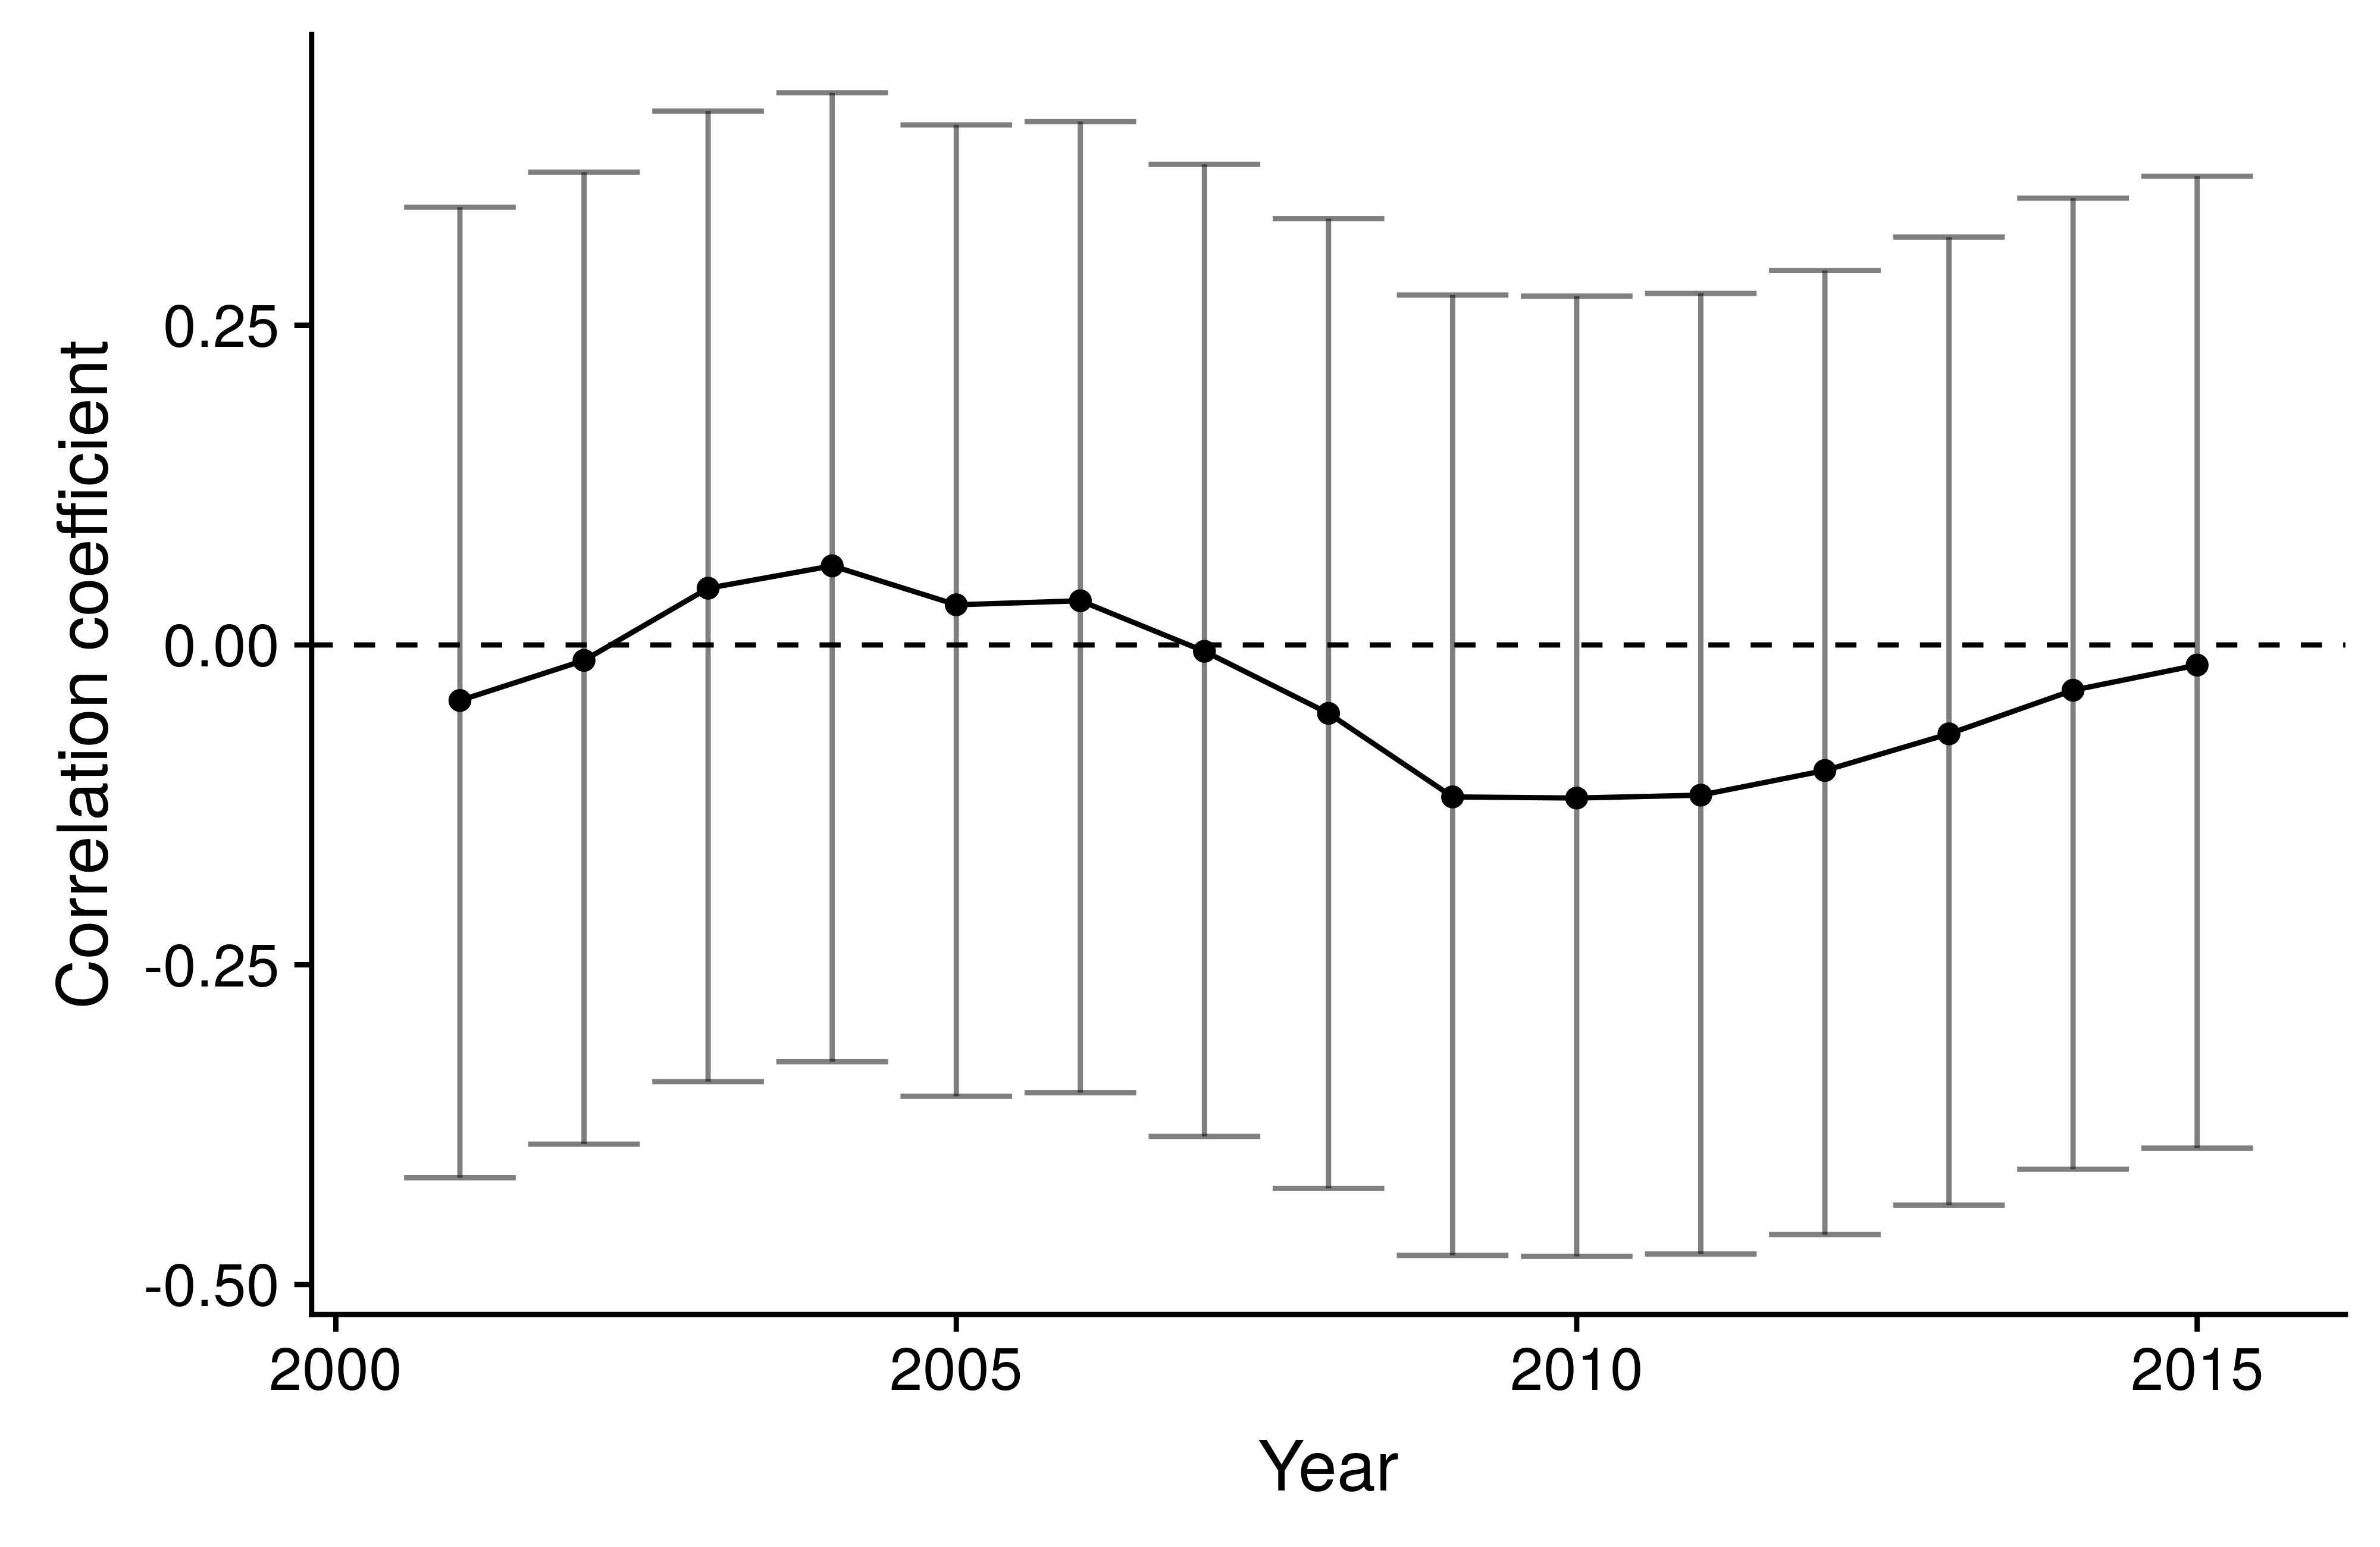
\includegraphics[width=.95\linewidth]{../figures/cor}
\caption{Pearson's product moment correlation coefficient with 95\% confidence intervals for year-specific association between GDP per Capita and Malaria prevalence.}
\label{fig:cor}
\end{figure}


\subsection*{Dumitrescu and Hurlin's panel Granger causality tests}

We sought to test the significance of the relationship between the prevalence of Malaria and GDP per Capita using a Granger Hypothesis test. According to Granger's theory of causality, if X causes Y, then past values of X should be predictive of future values of Y. Rather than a traditional Granger causality test, we used the approach outlined by Dumitrescu and Hurlin \cite{dumitrescu}, so as to exploit the panel nature of our data. We suspected that the relationship would be bi-directional (ie, that reductions in Malaria lead to economic growth and vice-versa), and anticipated that any differences in the effect size and significance level of the Granger causal association would be suggestive (but not demonstrative) of respectively greater directional causality.

We ran two tests: (A) with the null hypothesis that "Malaria decrease dot not cause GDP increase" and (B) with the null hypothesis that "GDP increase does not cause Malaria". The country-specific and aggregate test results are in table 1. The low P-value of test A suggests causality (or at least precedence), whereas the non-significant P-value of test B suggests that there is no case for temporal precedence. In other words, the Granger tests indicate that the Malaria-GDP pathway may be more important than the GDP-Malaria pathway.

The average Chi-squared values for the tests were 1.72 and 1.26, respectively. These values are comparable, given that they are run on paired vectors. Since the data consists of a balanced panel, we can also consider the Z-bar statistic, a reflection of the magnitude of the predictiveness, with scores of 2.63 and 0.94 for tests A and B, respectively.


\begin{table}

\caption{\label{tab:}Pangel Granger Causality test results}
\centering
\begin{tabular}[t]{lrr}
\toprule
Country & Chi-squared & P\\
\midrule
\addlinespace[0.3em]
\multicolumn{3}{l}{\textbf{A. Malaria decrease does not cause GDP increase | P=0.008}}\\
\hspace{1em}Angola & 0.887 & 0.346\\
\hspace{1em}Benin & 2.998 & 0.083\\
\hspace{1em}Burkina Faso & 6.007 & 0.014\\
\hspace{1em}Burundi & 0.225 & 0.635\\
\hspace{1em}Cameroon & 2.865 & 0.091\\
\hspace{1em}Central African Republic & 6.516 & 0.011\\
\hspace{1em}Congo, Dem. Rep. & 0.178 & 0.673\\
\hspace{1em}Congo, Rep. & 6.272 & 0.012\\
\hspace{1em}Cote d'Ivoire & 0.324 & 0.569\\
\hspace{1em}Gambia, The & 0.051 & 0.821\\
\hspace{1em}Ghana & 1.936 & 0.164\\
\hspace{1em}Guinea & 0.113 & 0.737\\
\hspace{1em}Guinea-Bissau & 0.133 & 0.715\\
\hspace{1em}Kenya & 0.005 & 0.944\\
\hspace{1em}Liberia & 2.339 & 0.126\\
\hspace{1em}Madagascar & 0.591 & 0.442\\
\hspace{1em}Malawi & 0.381 & 0.537\\
\hspace{1em}Mali & 0.052 & 0.820\\
\hspace{1em}Mozambique & 1.279 & 0.258\\
\hspace{1em}Nigeria & 0.549 & 0.459\\
\hspace{1em}Rwanda & 0.371 & 0.543\\
\hspace{1em}Senegal & 4.148 & 0.042\\
\hspace{1em}Sierra Leone & 4.821 & 0.028\\
\hspace{1em}Tanzania & 0.064 & 0.800\\
\hspace{1em}Togo & 2.950 & 0.086\\
\hspace{1em}Uganda & 0.120 & 0.729\\
\hspace{1em}Zambia & 0.179 & 0.672\\
\addlinespace[0.3em]
\multicolumn{3}{l}{\textbf{B. GDP increase does not cause Malaria decrease | P=0.346}}\\
\hspace{1em}Angola & 0.729 & 0.393\\
\hspace{1em}Benin & 0.016 & 0.899\\
\hspace{1em}Burkina Faso & 0.162 & 0.687\\
\hspace{1em}Burundi & 3.964 & 0.046\\
\hspace{1em}Cameroon & 0.115 & 0.735\\
\hspace{1em}Central African Republic & 2.929 & 0.087\\
\hspace{1em}Congo, Dem. Rep. & 0.072 & 0.789\\
\hspace{1em}Congo, Rep. & 0.016 & 0.899\\
\hspace{1em}Cote d'Ivoire & 3.366 & 0.067\\
\hspace{1em}Gambia, The & 4.068 & 0.044\\
\hspace{1em}Ghana & 0.020 & 0.888\\
\hspace{1em}Guinea & 0.282 & 0.595\\
\hspace{1em}Guinea-Bissau & 0.032 & 0.858\\
\hspace{1em}Kenya & 0.031 & 0.860\\
\hspace{1em}Liberia & 0.002 & 0.961\\
\hspace{1em}Madagascar & 1.575 & 0.210\\
\hspace{1em}Malawi & 4.963 & 0.026\\
\hspace{1em}Mali & 2.503 & 0.114\\
\hspace{1em}Mozambique & 1.786 & 0.181\\
\hspace{1em}Nigeria & 0.109 & 0.742\\
\hspace{1em}Rwanda & 1.416 & 0.234\\
\hspace{1em}Senegal & 0.061 & 0.804\\
\hspace{1em}Sierra Leone & 1.505 & 0.220\\
\hspace{1em}Tanzania & 0.911 & 0.340\\
\hspace{1em}Togo & 0.206 & 0.650\\
\hspace{1em}Uganda & 2.175 & 0.140\\
\hspace{1em}Zambia & 0.908 & 0.341\\
\bottomrule
\multicolumn{3}{l}{\textsuperscript{*} Country-specific Granger causality test values. The null}\\
\multicolumn{3}{l}{hypotheses (in bold) preceding each section can be}\\
\multicolumn{3}{l}{rejected at a P-value of less than 0.05, both at the}\\
\multicolumn{3}{l}{individual country level, or as the aggregate Granger test}\\
\multicolumn{3}{l}{statistic (also in bold).}\\
\end{tabular}
\end{table}



\subsection*{Bruckner's 2-step model}

Our Granger tests are suggestive of a health to wealth causal pathway, but not the opposite. We take these findings to be indicative of the greater magnitude of the health to wealth pathway relative to the wealth to health pathway. However, we do not rule out the latter, since (i) our inability to reject the null hypothesis may be somewhat a function of small sample size and (ii) other studies have found a plausible wealth to health pathway in a number of settings.

Accordingly, we employ a two-step least squares approach, as per Bruckner \cite{bruckner2011}, to adjust for the potential effect of GDP growth on the prevalence of Malaria. For estimating changes in GDP, we use ITN coverage, which should have a significant effect on malaria but not on GDP growth (except for its indirect effect via Malaria's reduction), as an instrumental variable. Having estimated the effect of lagged log changes in GDP on Malaria, we can then use the residual variation in Malaria prevalence which is not explained by GDP to estimate the effect of Malaria on GDP growth. Inversely, for changes in Malaria, we use consumer gasoline prices as our IV, which should have an effect on GDP grwoth but not on malaria (except for via GDP). Having estimated the effect of lagged log changes in Malaria's prevalence on GDP, we then use the residual variation in GDP which is not explained by Malaria prevalence to estimate the ffect of GDP growth on Malaria. 

Table 2 shows the model results for both the first (IV) and second steps. Since the causal pathways are endogenous, the results of the second step are more indicative of causality than those of the first. The significance of ITN on GDP growth, after adjustment for the variance in Malaria's prevalence which can be explained by GDP suggests a causal pathway from a reduction in Malaria to an increase in GDP per capita, and is consistent with the similar precednet pathway detected via Granger analysis.  


\begin{table}

\caption{\label{tab:}Results of Bruckner second-step models}
\centering
\begin{tabular}[t]{lllrrr}
\toprule
Step & Pathway & Coefficient & Estimate & S.E. & P-value\\
\midrule
1 & Wealth to health (IV) & GDP & 0.000 & 0.000 & 0.402\\
 &  & IV (ITN) & 0.028 & 0.049 & 0.564\\
 & Health to wealth (IV) & Malaria & 0.073 & 0.123 & 0.550\\
 &  & IV (gas) & -0.173 & 0.062 & 0.006\\
2 & Health to wealth & IV (ITN) & -0.183 & 0.061 & 0.003\\
 &  & IV residuals & 0.120 & 0.114 & 0.292\\
 & Wealth to health & IV (gas) & 0.024 & 0.049 & 0.625\\
 &  & IV residuals & 0.067 & 0.070 & 0.340\\
\bottomrule
\multicolumn{6}{l}{\textsuperscript{*} In step 2, "Health to wealth" refers to the lagged log changes in the}\\
\multicolumn{6}{l}{prevalence of Malaria on relative log changes in growth in GDP per}\\
\multicolumn{6}{l}{capita; "Wealth to health" refers to the inverse.}\\
\end{tabular}
\end{table}



\subsection*{Robustness checks}

Our results show coherent evidence for the primacy of the Malaria reduction to GDP growth causal pathway over the inverse. Whereas Granger analysis establishes the temporal precedence required of a causal relationship, Brückner's two-step instrument approach provides further evidence. Though results point in the same direction, neither method can be considered "proof" of causality. Accordingly, we test the extent to which the health to wealth theory holds up under different conditions and scenarios, so as to provide further evidence of causal directionality, or qualify/refute such causality. 

\textbf{Artemisinin-based combination therapy (ACT)} was introduced in 2005, but not uniformly across Africa, offering an ideal natural experiment wherein one can examine the effect on GDP of an exogenous shock to health (via improved malaria treatment). Though ACT affects already infected individuals, rather than preventing infection itself, the associated reduction in morbidity should have directionaly similar economic consequences as a reduction in prevalence. Therefore, given the previously identified health to wealth theory, we expect the introduction of ACT to be associated with a subsequent increase in GDP per capita. We defined "introduction" as greater than 10\% of febrile cases among children under 5 being treated with ACT. Figure 3 shows the trends in country-specific GDP per capita as a percentage of the year prior to ACT introduction for all countries where ACT was introduced.


\begin{figure}%[tbhp] Remove the asterisk to get column width only
\centering
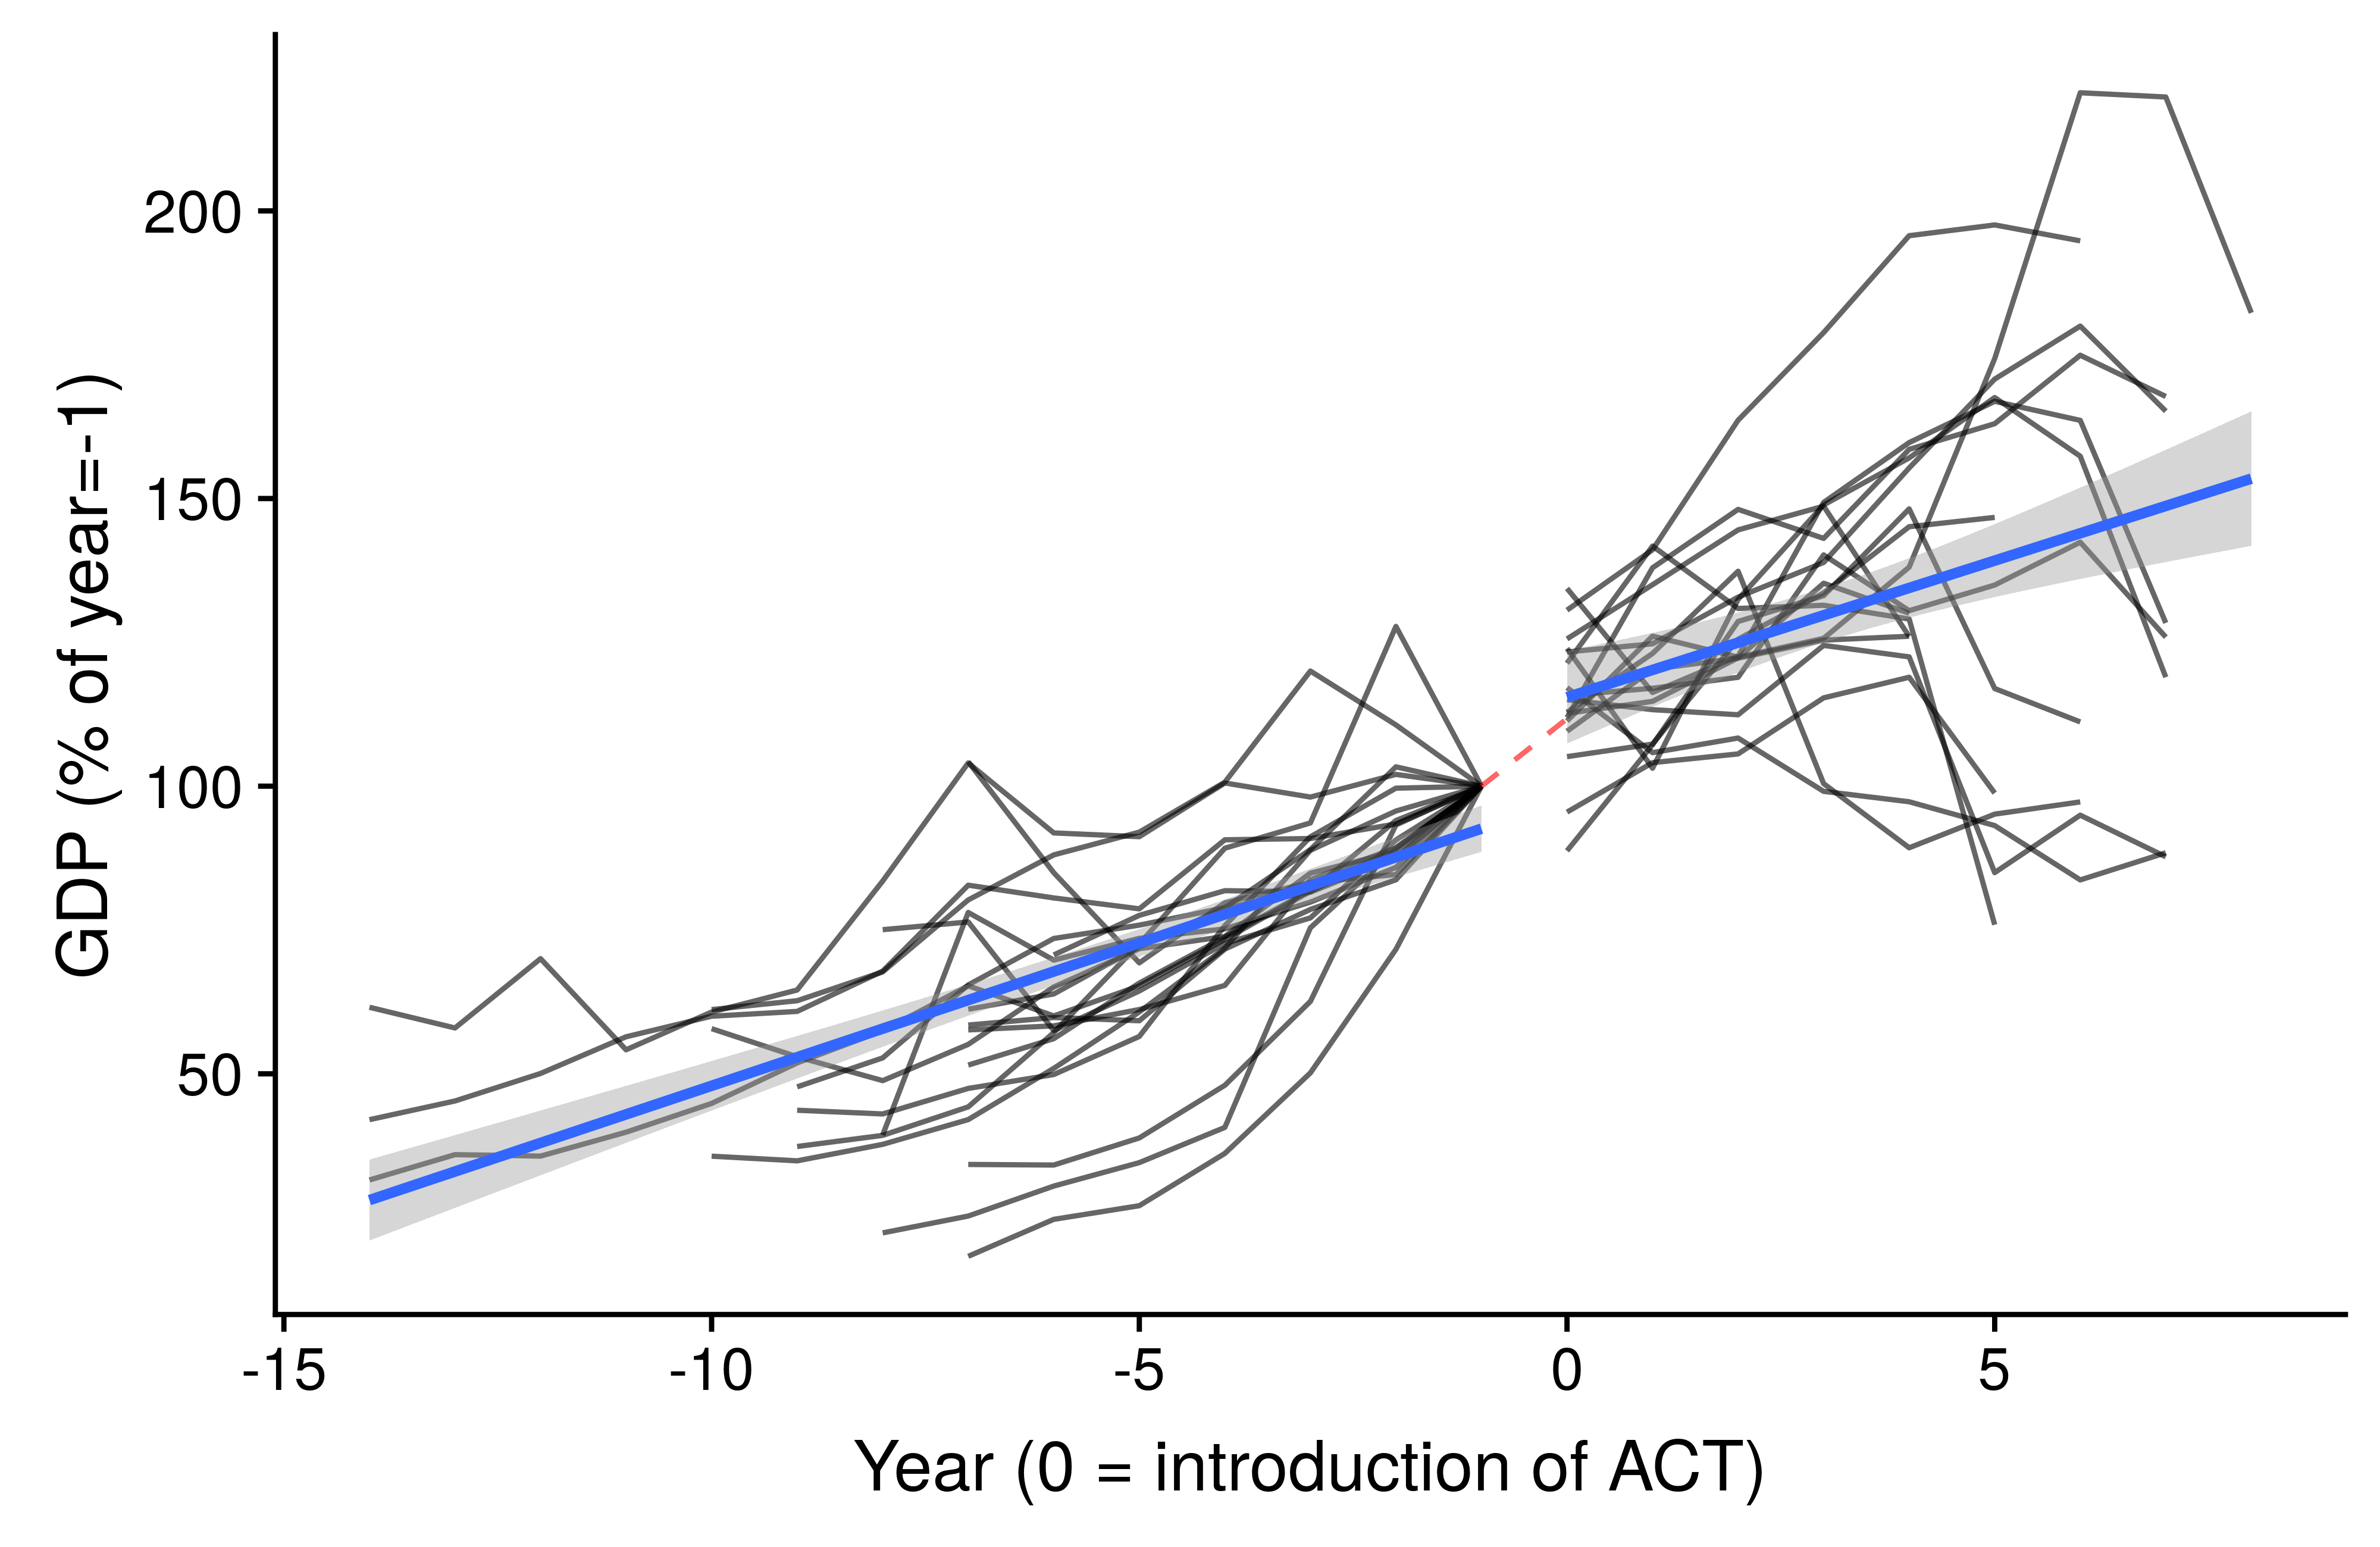
\includegraphics[width=.95\linewidth]{../figures/act}
\caption{Impact of introduction of ACT (ACT coverage > 10\%) on GDP growth in high-endemicity African countries}
\label{fig:act}
\end{figure}

The slope for the post post-ACT trend line is stiatistically similar to that of the pre-ACT period (95\% confidence intervals of 4.21-5.73 and 2.60-6.90, respectively). However, the change in intercept between the two fitted lines is of large magnitude: on average, the year of ACT introduction is associated with a 12\% greater GDP per capita than the prior year, well outside the range predicted by the pre-ACT trend. In other words, the introduction of ACT is associated with a significantly larger than normal growth in GDP per capita, an association consistent with our results.

\textbf{The 2008 financial crisis} saw a dip in GDP per capita among many African countries. Of the 27 countries we examined, 19 (70.3\%) had their economies shrink from 2008 to 2009. A health to wealth causal pathway would suggest that we should see a significant increase in the prevalence of Malaria in the period following the crisis. Figure 4 shows the association between the change in GDP per capita between 2008-9 and the relative reduction in malaria both for 2008-9 as well as the following year.

\begin{figure}%[tbhp] Remove the asterisk to get column width only
\centering
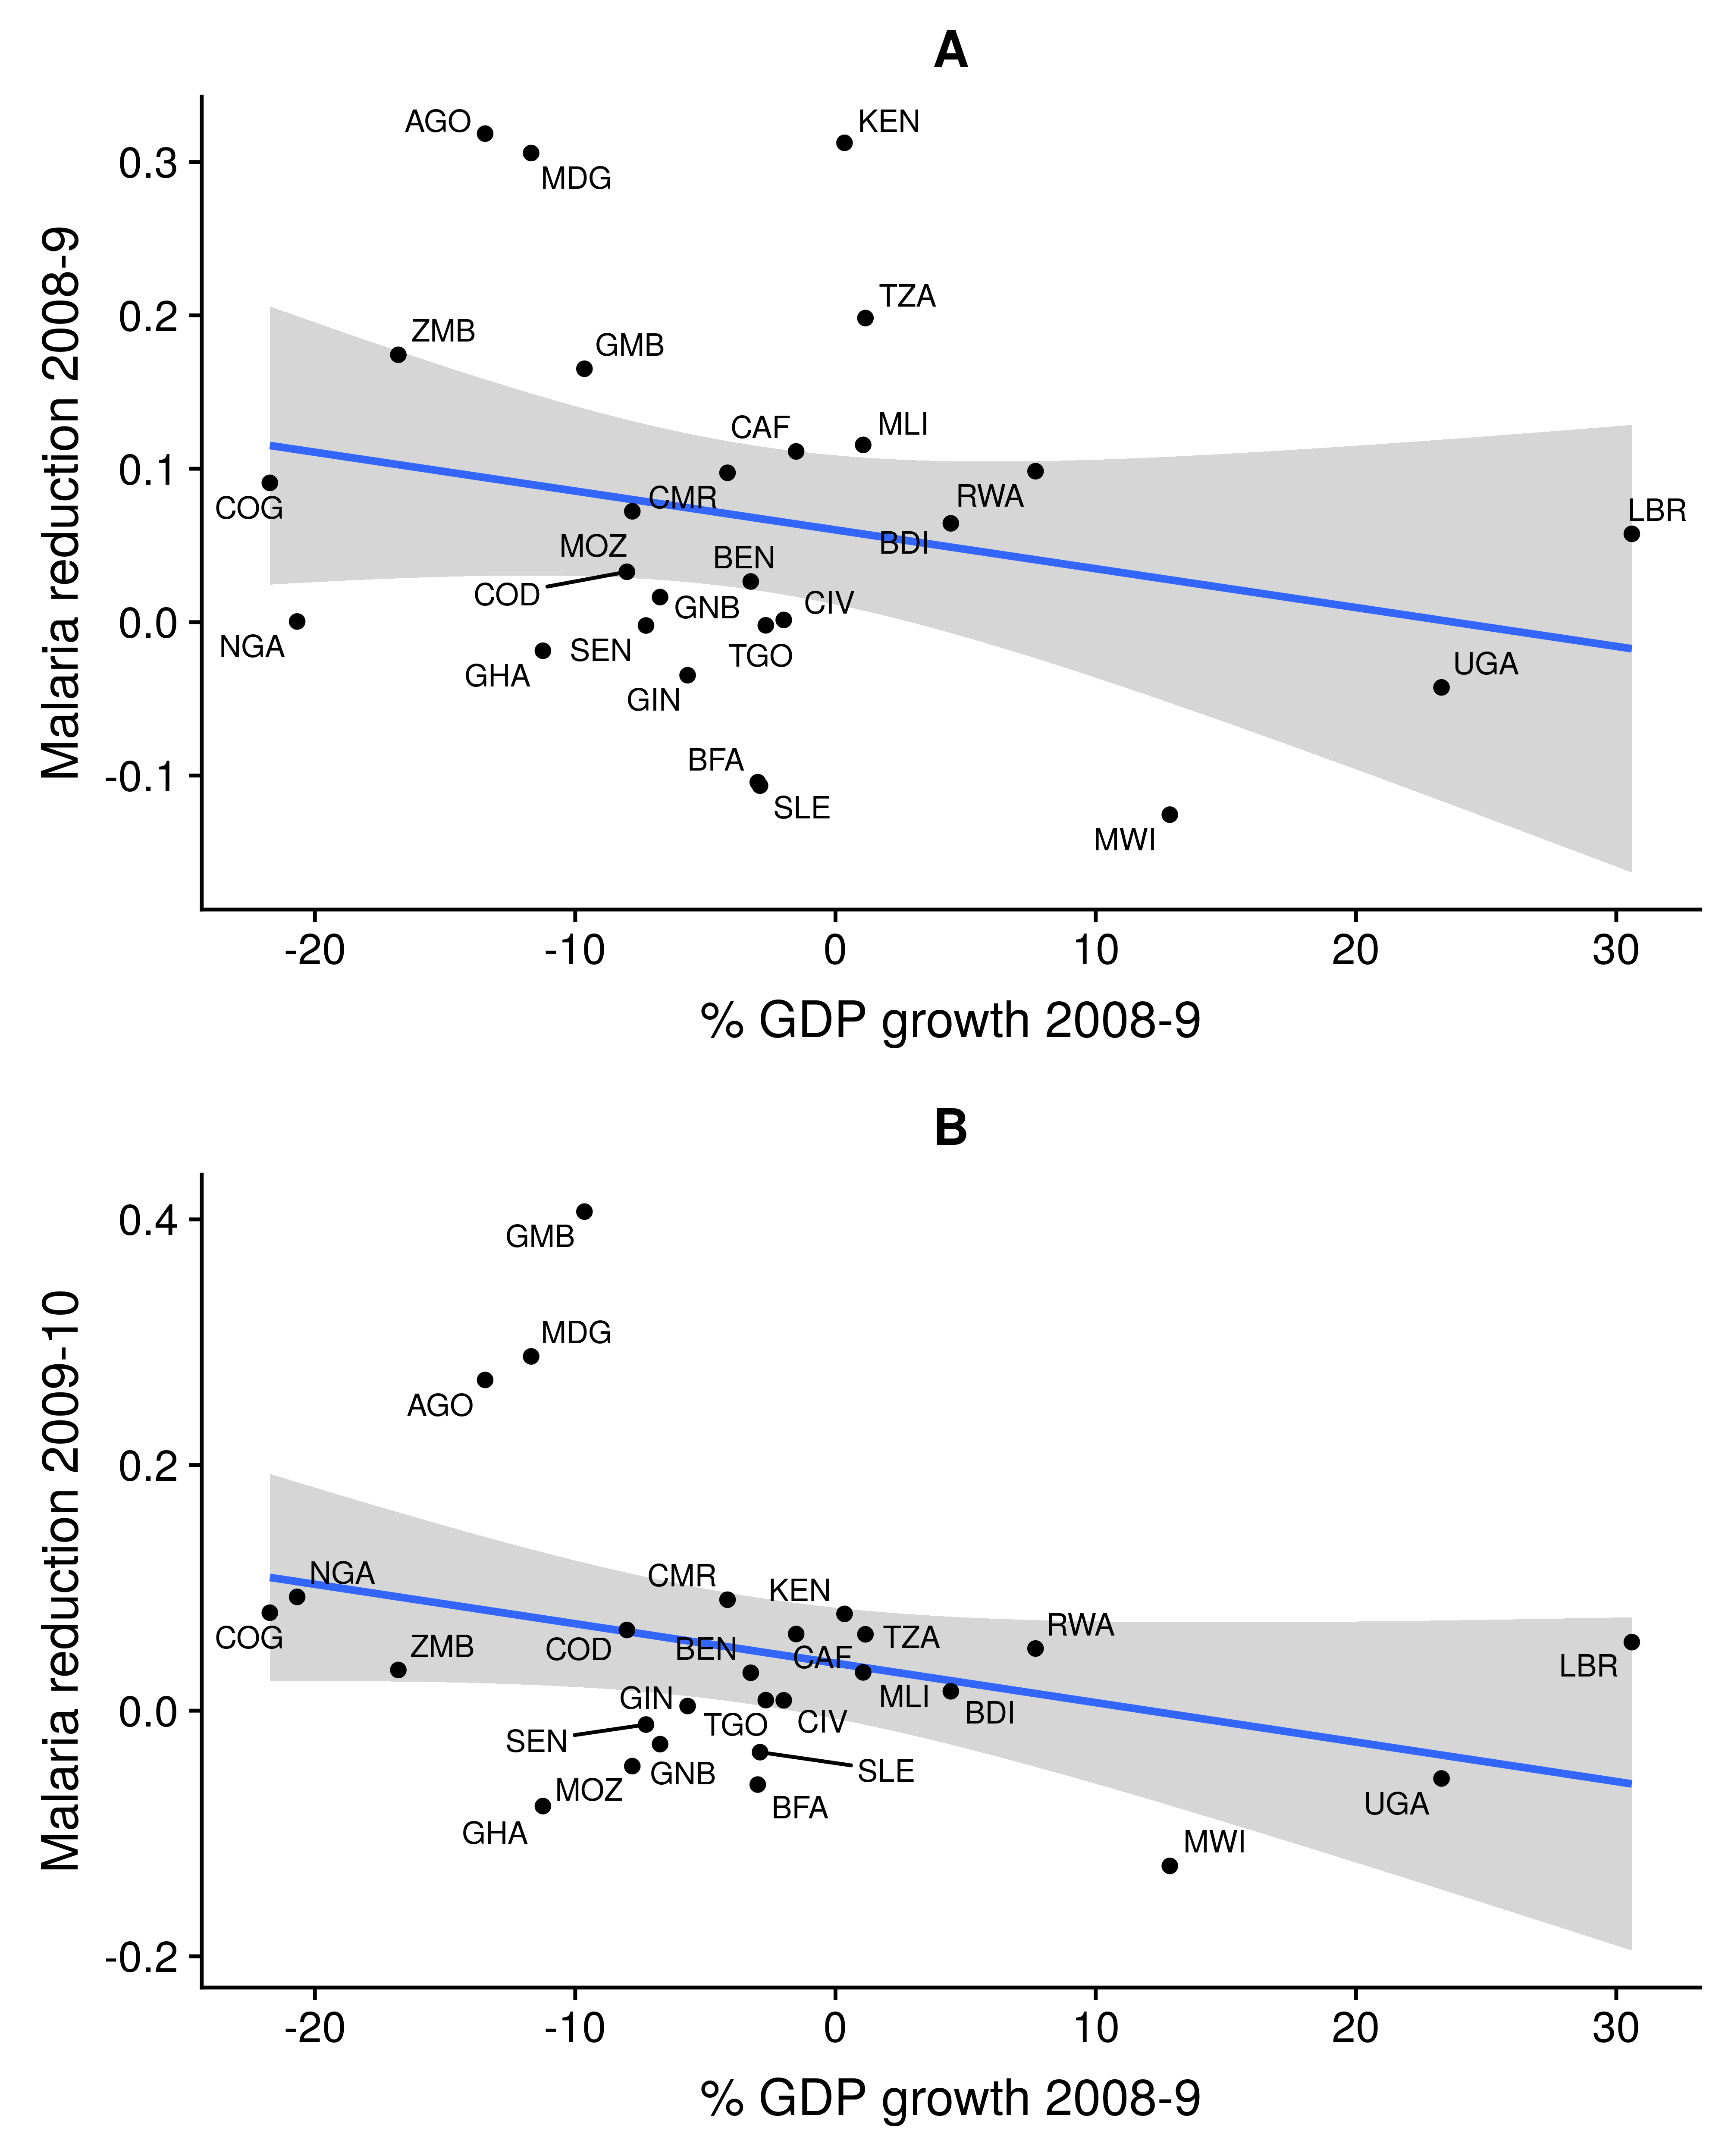
\includegraphics[width=.95\linewidth]{../figures/crisis}
\caption{Association of growth in GDP per capita and Malaria reduction during the global financial crisis. The line of best fit (OLS) is in blue.}
\label{fig:act}
\end{figure}

On average, the countries most affected by the financial crisis also saw the greatest reductions in Malaria during and immediately following the crisis. This is inconsistent with a wealth to health causal pathway, again supporting our health to wealth primacy theory.



\section*{Discussion}

In our analysis, we examined 27 Sub-Saharan African countries over a 15 year period and found greater evidence for a causal health to wealth pathway - at least in terms of malaria - than the opposite. 

Our findings are consistent with several previous studies. Chen found a bi-directional health-wealth relationship \cite{Chen_2013}, as did Erdil and Yetkiner, the latter showing that health to wealth one-way causal plausability was greatest in the case of low and middle income countries \cite{Erdil_2009}. 

Most previous research focuses on the relationship between GDP and health spending (rather than outcomes). When research has been directed out outcomes, studies have largely remained general rather than looking at the effect of a specific disease; Audibert examined the relationship between GDP and DALYs among a mix of high and low income countries, and also found evidence for a causal health to wealth pathway. In regards to Malaria's effect, Orem examined Ugandan malaria morbidity data and GDP growth on a much more granular scale (albeit only one country and during only a 7 year period), and found a significant effect of health on wealth \cite{Orem_2012}. This is the first study, to the authors' knowledge, which examines Malaria-specific outcomes (prevalence) and interventions (ACT and ITN) in regards to their effect on GDP across multiple countries.

This study has several limitations. First, it does not report on the effect of inequality on growth, though this could be a confounding factor in the relationship between growth and Malaria \cite{Asafu_Adjaye_2004}. Second, the countries in our observation pool are relatively uniform in that nearly all carried out malaria control programs and experienced overall economic growth. The extent to which are findings are generalizable to other contexts is unknown. Additionally, the relatively short nature of our study period (15 years) prohibited any estimation of the long-term "snowballing" accumulation of health and wealth benefits, potentially resulting in the unintentional underestimation of both. Finally, though we restricted our analysis to countries which had a high burden of Malaria at the beginning of the study period, we did not examine the differential effect of reductions in Malaria on GDP as a function of the baseline prevalence.

Nonetheless, our results offer compelling evidence that reductions in Malaria are causally associated with economic growth. A country's health and wealth are intimately correlated, particularly in areas with a disease as debilitating and prevalent as Malaria. Policymakers and development workers should take into account the health to wealth pathway when planning interventions, and consider targeting Malaria directly through public health interventions as a means to not only improved health but also economic growth.



\matmethods{Data on the estimated Plasmodium falciparum parasite rate in 2-10 year olds from the period from 2000 through 2015 was obtained from the Malaria Atlas Project \cite{Hay_2006, Guerra_2007}. Annual Gross Domestic Product (GDP) per capita data was obtained from the World Bank \cite{worldbank}. We used the raster package \cite{raster} to aggregate point-specific Pf rates into annual country-wide averages (henceforth referred to as "Malaria prevalence"). All data processing and analysis was carried out in R \cite{rr}, and all data and code are freely available online \cite{brew}. Following the construction of our panel dataset, we used the PML package for the estimation of our Granger causality models \cite{Croissant_2008}.}

\showmatmethods % Display the Materials and Methods section

\pnasbreak


% Bibliography
\bibliography{pnas-sample}

\end{document}